\documentclass[a4paper, 14pt]{extarticle}



\usepackage[main=russian,english]{babel}   %% загружает пакет многоязыковой вёрстки
\usepackage{fontspec}      %% подготавливает загрузку шрифтов Open Type, True Type и др.

\setmainfont{Times New Roman}
\setsansfont{Times New Roman}

\usepackage{icomma}
\usepackage{siunitx}
\usepackage[a4paper,top=1cm,bottom=2cm,left=3cm,right=1.5cm, marginparwidth=2cm]{geometry}

\usepackage{graphicx}
\usepackage{amsmath, amsfonts}
\usepackage{longtable}
\usepackage{icomma}
\usepackage{indentfirst}


\usepackage{mathrsfs}
\usepackage{xcolor}
\usepackage{hyperref}
\usepackage{enumitem}
\usepackage[export]{adjustbox}

\input{../include/definitions.inc}

\begin{document}
	
	
\section{Плоские потенциальные течения идеальной жидкости и комплексные потенциалы}



\subsection{Построение комплексного потенциала плоского потенциального течения идеальной жидкости }

Если возможно ввести систему координат так, что течение идеальной жидкости ($\rho=const$) будет описываться уравнениями:	
\begin{equation}
	\label{eq:ideal_liquid_planar_mass}
	\pd{v_x}{x}+\pd{v_y}{y} = 0,
\end{equation}
\begin{equation}
	\label{eq:ideal_liquid_planar_momentum_x}
	\pd{v_x}{t}+v_x \pd{v_x}{x} + v_y \pd{v_x}{y} = -\frac{1}{\rho} \pd{p}{x},
\end{equation}	
\begin{equation}
	\label{eq:ideal_liquid_planar_momentum_y}
	\pd{v_y}{t}+v_x \pd{v_y}{x} + v_y \pd{v_y}{y} = -\frac{1}{\rho} \pd{p}{y},	
\end{equation}
где $v_x = v_x(t,x,y)$, $v_y = v_y(t,x,y)$, $p=p(t,x,y)$ -- функции, заданные в некоторой исследуемой области, то говорят, что движение идеальной жидкости \textit{плоскопараллельное}.

\begin{dfn}
	Функция $\psi=\psi(x,y)$ такая, что 
	\[
	v_x = \pd{\psi}{y},\quad
	-v_y = \pd{\psi}{x},
	\]
	называется функцией тока. Если течение нестационарное, то $t$ -- дополнительный параметр.
\end{dfn}

Для функции $\psi = \psi(x,y)$ уравнение неразрывности (\ref{eq:ideal_liquid_planar_mass})
\[
	\pd{v_x}{x} + \pd{v_y}{y} = 
	\pd{}{x} \left( \pd{\psi}{y} \right) + \pd{}{y} \left( -\pd{\psi}{x} \right) = 0
\]
выполняется тождественно.


Рассмотрим уравнения \textit{линий тока}:
\[
	\frac{dx}{v_x(x,y)} = \frac{dy}{v_y(x,y)},
\]
тогда
\[
0 = -v_y dx + v_x dy = \pd{\psi}{x} dx + \pd{\psi}{y} dy =  d\psi.
\]
Таким образом, $\psi=\psi(x,y)$ \textit{сохраняет} одно и то же значение \textit{на линиях тока}.
		
Вектор вихря $\vec{\Omega}= \rot \vec{v}$ задается формулами:
\[
	\Omega_x = \pd{v_z}{y}-\pd{v_y}{z} = 0,\quad
	\Omega_y = \pd{v_x}{z}-\pd{v_z}{x} = 0,
\]
\[
	\Omega_z = \pd{v_y}{x}-\pd{v_x}{y} = -\pdk{\psi}{x} - \pdk{\psi}{y}.
\]
		
В случае безвихревого течения ($\vec{\Omega} = 0$):
\[
	\Delta \psi = \pdk{\psi}{x} + \pdk{\psi}{y} = 0.
\]


Если плоское течение идеальной жидкости \textit{потенциально}, тогда существует функция $\varphi(x,y)$ такая, что
\[
	v_x = \pd{\varphi}{x},\quad
	v_y = \pd{\varphi}{y}, 
\]
при этом
\begin{equation}
	\label{eq:Cauchi_Riman}
	\pd{\psi}{y} = \pd{\varphi}{x},\quad
	-\pd{\psi}{x} = \pd{\varphi}{y}.
\end{equation}
	
Иначе,
\[
\pd{\varphi}{x}\pd{\psi}{x} + \pd{\varphi}{y}\pd{\psi}{y} = 0.
\]
Отсюда следует, что линии $\varphi=const$ и $\psi=const$ \textit{ортогональны}. Такие $\varphi$ и $\psi$ называются \textit{сопряженными}.
		
	
Функции $\varphi$ и $\psi$ связаны между собой условием Коши -- Римана (\ref{eq:Cauchi_Riman}), поэтому функция комплексного переменного $w(z) = \varphi(x,y) + i \psi(x,y)$ является \textit{аналитической функцией} комплексного аргумента $z = x + i y$:
\begin{equation}
	\label{eq:complex_potential_dfn}
	w(z) = f(x+iy) = \varphi(x,y) + i  \psi(x,y).
\end{equation}

\begin{dfn}
	Функция $w(z)$ (\ref{eq:complex_potential_dfn}) называется \textit{комплексным потенциалом} плоскопараллельного потенциального течения идеальной жидкости.
\end{dfn}			
		
		
\begin{dfn}
	Комплексная функция $v(z)$, определенная по формуле
	\[
	v(z) = v_x(x,y) + i v_y(x,y),
	\] 
	называется  \textit{комплексной скоростью} (см. рис. \ref{fig:v_complex_dfn}).
\end{dfn}

Так как $w(z)$ -- аналитическая функция, то существует $dw/dz$:
\[
\od{w}{z} = \pd{\varphi}{x}+\pd{\psi}{x} i = 
\pd{\varphi}{x}-\pd{\varphi}{y} i = v_x-i v_y = v^*. 
\]

\begin{figure}
	\centering
	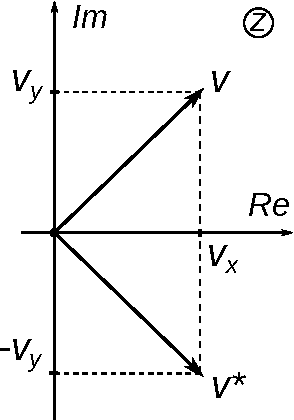
\includegraphics[width=0.3\linewidth]{../img/v_star.pdf}
	\caption{Определение комплексной скорости и её комплексно-сопряжённой величины}
	\label{fig:v_complex_dfn}
\end{figure}
					
Связь \textit{плоской потенциальной гидродинамической задачи} с теорией функций комплексного переменного (ТФКП) заключается в том, что соотношение
\[
w(z) = f(x+iy) = \varphi(x,y) + i  \psi(x,y)
\]
связывает аналитическую функцию $w(z)$ с определённой кинематической картиной течения и полем ($v_x$, $v_y$) с помощью аппарата ТФКП и наоборот.

\bigskip
Рассмотрим простейшие примеры.

\begin{problems}
\item 
\textbf{Однородное поступательное течение.}
Комплексный потенциал:
\[
	w(z) = a z,\quad
	a \in\mathbb{R}.
\]
		
Комплексная скорость:
\[
	\od{w}{z} = a = v_x - i v_y \Rightarrow
	v_x = a,\quad v_y = 0.
\]

Линии тока этого течения (при $a>0$) изображены на рис. \ref{fig:uniform_translation}.

\begin{figure}
	\centering
	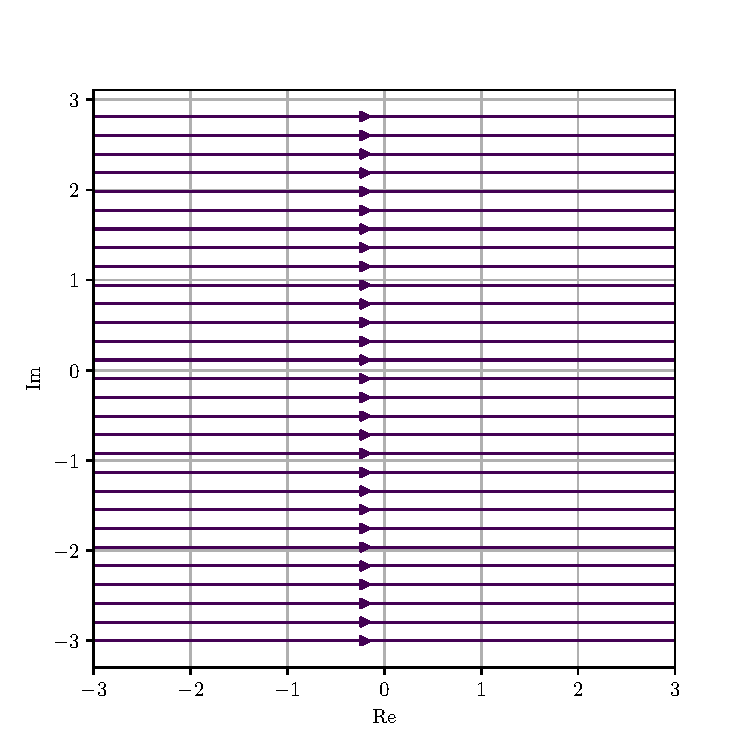
\includegraphics[width=0.45\textwidth]{../img/uniform_translation.pdf}
	\caption{Линии тока однородного поступательного движения при $a>0$}
	\label{fig:uniform_translation}
\end{figure}


\item 
\textbf{Источник и сток.} Комплексный потенциал:
\[
	w(z) = \frac{q}{2\pi}\ln(z-z_0),\quad
	q \in\mathbb{R}, z_0\in\mathbb{C}.
\]
			
Пусть $z=x+iy=re^{i\theta}$, тогда комплексная скорость (при $z_0 = 0$) имеет вид:
\[
\od{w}{z} = \frac{q}{2\pi}\frac{1}{z} \Rightarrow
\left\{
\begin{array}{l}
\displaystyle v_x = \frac{q}{2 \pi}\frac{x}{x^2+y^2} = \frac{q}{2\pi r}\cos\theta,\\
\displaystyle v_y = \frac{q}{2 \pi}\frac{y}{x^2+y^2} = \frac{q}{2\pi r}\sin\theta.
\end{array}
\right.
\]


Линии тока этого течения изображены на рис. \ref{fig:source_sink}.

\begin{figure}
	\centering
	\begin{tabular}{cc}
	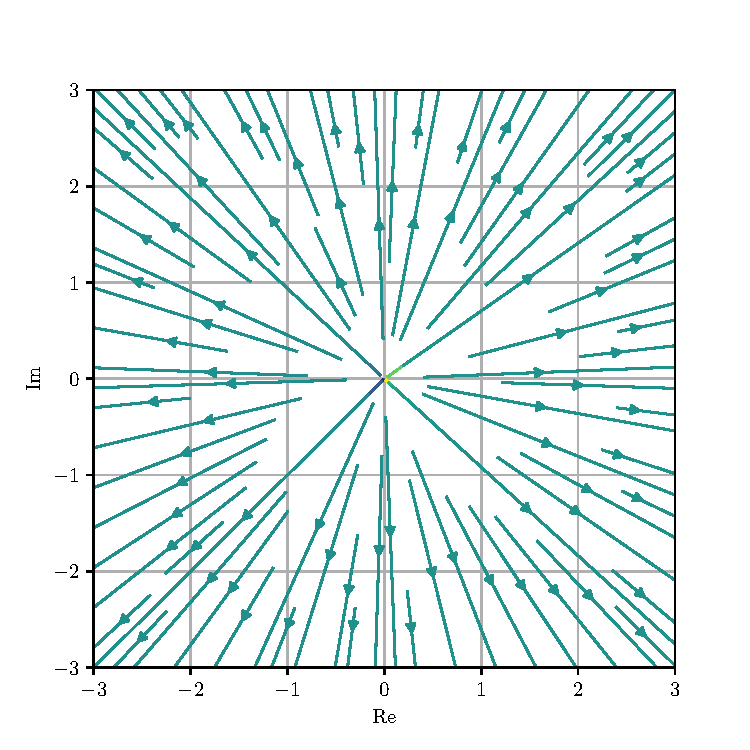
\includegraphics[width=0.45\textwidth]{../img/source.pdf} &
	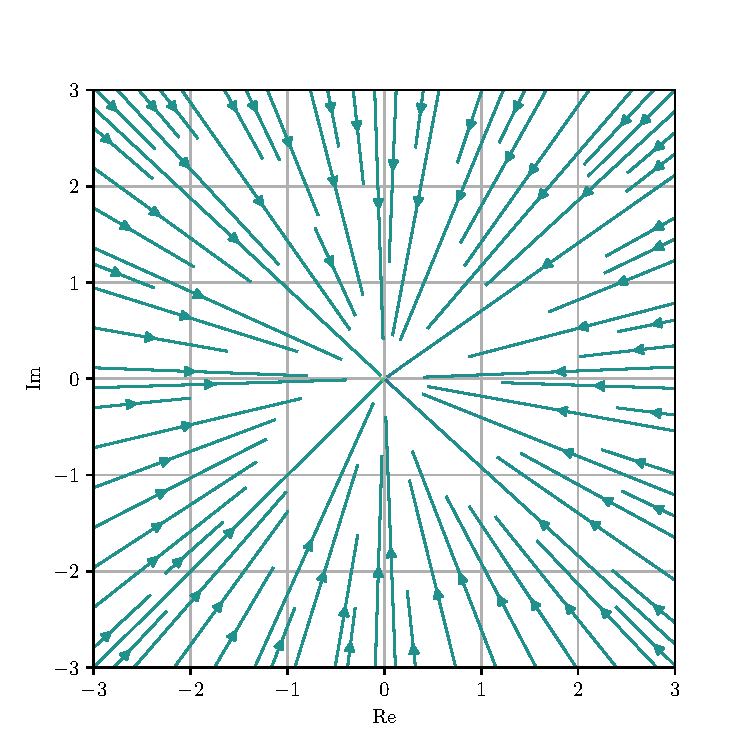
\includegraphics[width=0.45\textwidth]{../img/sink.pdf} \\
	а & б 
	\end{tabular}
	\caption{Линии тока источника ($q>0$) (a) и стока ($q<0$) (б)}
	\label{fig:source_sink}
\end{figure}

\item
\textbf{Вихрь.} Комплексный потенциал:
\[
	w(z) = \frac{\Gamma}{2\pi i}\ln(z-z_0),\quad
	\Gamma \in\mathbb{R}, z_0\in\mathbb{C}.
\]
			
Пусть $z=x+iy=re^{i\theta}$, тогда комплексная скорость (при $z_0=0$):
\[
	\od{w}{z} = \frac{\Gamma}{2\pi i}\frac{1}{z} \Rightarrow 
	\left\{
	\begin{array}{l}
		\displaystyle	v_x = -\frac{\Gamma}{2\pi}\frac{y}{x^2+y^2} = -\frac{\Gamma}{2\pi r}\sin\theta,\\
		\displaystyle	v_y = \frac{\Gamma}{2\pi}\frac{x}{x^2+y^2} = \frac{\Gamma}{2\pi r}\cos\theta.
	\end{array}
	\right.
\]

Линии тока этого течения изображены на рис. \ref{fig:rotor}.

\begin{figure}
	\centering
	\begin{tabular}{cc}
		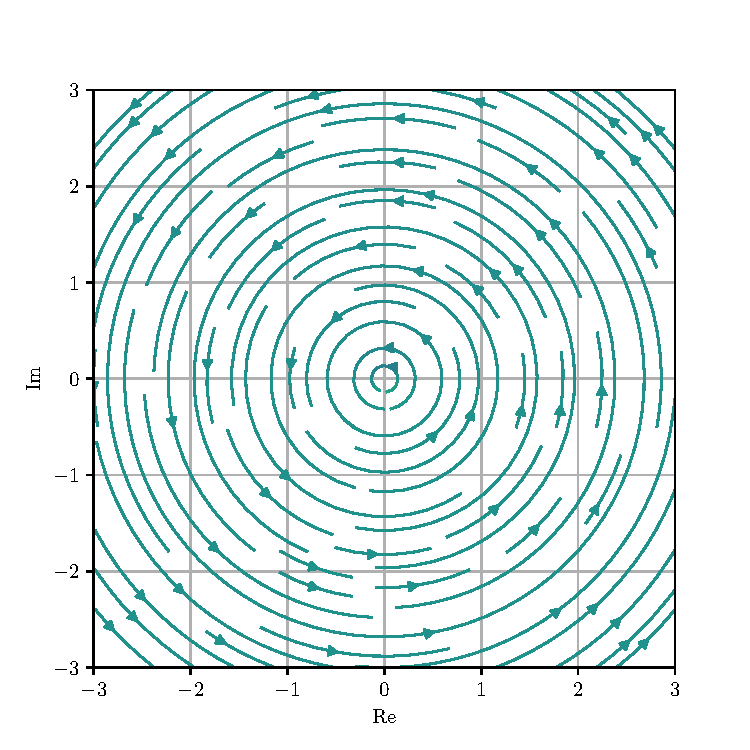
\includegraphics[width=0.45\linewidth]{../img/rot_Gamma_g_0.pdf} &
		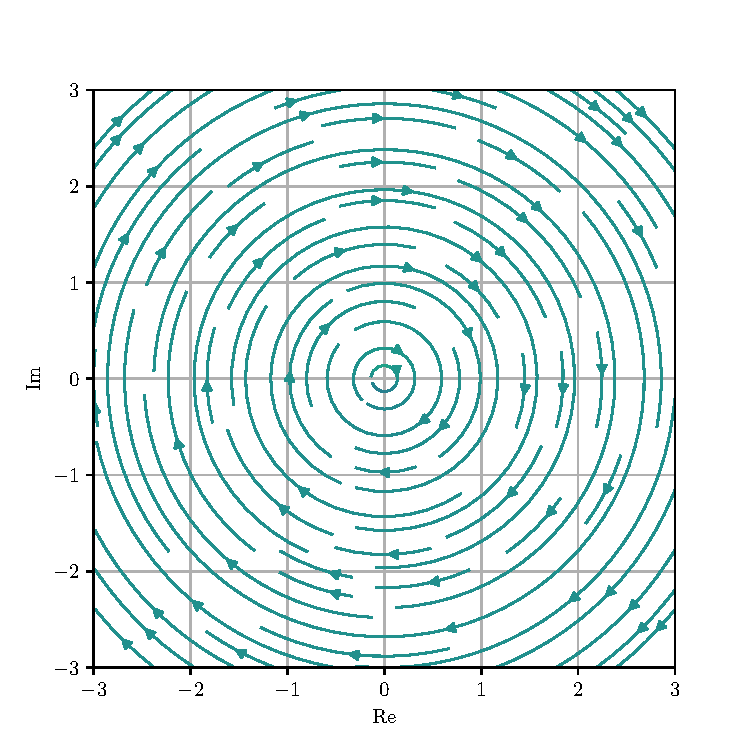
\includegraphics[width=0.45\linewidth]{../img/rot_Gamma_l_0.pdf} \\
		а & б 
	\end{tabular}
	\caption{Линии тока вихря, вращающегося в положительном ($\Gamma > 0$) (a) и отрицательном ($\Gamma < 0$) (б) направлениях}
	\label{fig:rotor}
\end{figure}

\item
\textbf{Диполь.}		
Комплексный потенциал:
\[
	w(z) = \frac{D e^{i\alpha}}{2\pi z},\quad
	D,\alpha \in\mathbb{R}.
\]
						
Пусть $z=x+iy=re^{i\theta}$, тогда комплексная скорость (при $\alpha=0$):
\[
	\od{w}{z} = -\frac{D}{2\pi}\frac{1}{z^2} \Rightarrow\displaystyle
	\left\{
	\begin{array}{l}
		v_x = -\displaystyle\frac{D}{2\pi r^2} \cos 2\theta,\\
		v_y = -\displaystyle\frac{D}{2\pi r^2} \sin 2\theta.
	\end{array}
	\right.
\]

Линии тока этого течения изображены на рис. \ref{fig:dipol}.

\begin{figure}
	\centering
	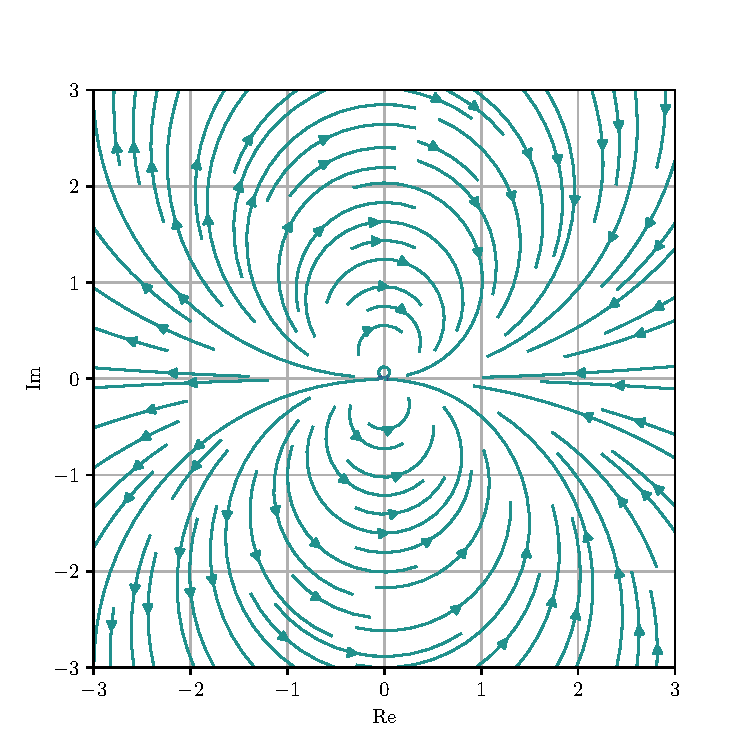
\includegraphics[width=0.45\linewidth]{../img/dipol.pdf}
	\caption{Линии тока диполя при $D>0$ и $\alpha = 0$}
	\label{fig:dipol}
\end{figure}
\end{problems}

\subsection{Построение потенциалов сложных течений}

Для моделирования течений, в которых присутствуют источники, стоки и другие элементарные течения применяется \textit{принцип суперпозиций}, заключающийся в следующем утверждении. Вследствие линейности уравнения неразрывности, если в области имеется несколько течений с потенциалами $w_1(z)$, $w_2(z)$, \ldots , $w_n(z)$, то общий потенциал всего течения в заданной точке равен сумме потенциалов всех течений, присутствующих в области:
\[
w(z) = w_1(z) + w_2(z) + \ldots + w_n(z).
\] 


Ещё один способ построения аналитических функций, описывающих плоские потенциальные течения ---  использовать \textit{метод конформных отображений} и \textit{теорему Римана о конформном отображение односвязных областей}. 

Основная идея заключается в построении конформного отображение физической плоскости $z$  на вспомогательную плоскость $\zeta$  с помощью аналитической функции $z=f(\zeta)$. Причём предполагается, что потенциал течения на вспомогательной плоскости известен $\psi(\zeta)$. Тогда искомый потенциал течения в физической плоскости  $\chi(z)$ будет выражаться из уравнений:
\[
\left\{
\begin{array}{l}
	\chi = \chi(f(\zeta)) = \psi(\zeta),\\
	z = f(\zeta).
\end{array}
\right.
\]
В этом случае комплексная скорость может быть найдена по формуле:
\[
v^* = \od{\chi}{z} = \od{\psi}{\zeta}  \od{\zeta}{z}.
\]


\subsection{Вычисление реакций и моментов сил, действующих на тело, при плоском потенциальном обтекании}
	

			
Для вычисления сил, моментов сил, действующих на выделенные контуры внутри области плоского потенциального течения, используют \textit{формулы Блазиуса -- Чаплыгина}:
\[
R^* = X - i Y = \frac{i\rho}{2} \oint\limits_C \left(\od{w}{z} \right)^2 dz,
\]	
\[
L = \Re \left[
-\frac{\rho}{2}\oint\limits_C \left(\od{w}{z} \right)^2 zdz
\right],
\]
где $R=X+i Y$ -- комплексная сила; $L$ -- величина главного момента; $\rho$ -- плотность жидкости; $C$ -- контур внутри или на границе области течения.

Также для вычисления реакций и момента главных сил можно использовать \textit{формулы Кутты -- Жуковского}. Если поток потенциален вне тела, которое можно заменить на конечное число источников, вихрей и диполей, лежащих внутри границы тела -- контура $C$, то
\[
R^* =  X - iY = i\rho\Gamma v_\infty^*,		
\]
\[
L = \Re \left[
-\rho v_\infty^*\sum\limits_{k=1}^m\Gamma_kb_k-i\rho M v_\infty^*
\right],
\]
где
$\Gamma_i$ -- циркуляции вихрей, находящихся в точках $b_i$ $(i=1,\ldots,m)$; $M$ -- суммарный момент источников и диполей; $\Gamma$ -- суммарная циркуляция вихрей, находящихся внутри тела.



\subsection{Задачи для самостоятельного решения}

\begin{problems}

	\item Установить связь функции тока с линиями тока.

	\item Рассмотреть плоское течение идеальной жидкости, задаваемое комплексным потенциалом $w(z) = Cz$, где $C = |C| e^{i \alpha}$.

	\item Для заданных комплексных потенциалов плоского течения идеальной жидкости:
		\begin{enumerate}
			\item 
			$
				w(z) = \ln \left( z^2 + \displaystyle\frac{1}{z^2} \right),
			$
			\item 
			$ 
			w(z) = \ln \left( 1 + \displaystyle\frac{1}{z^2} \right),
			$
		\end{enumerate}
	найти обильность $Q$ и построить качественную картину течения.
	
	\item 
	Границы какого геометрического объекта обтекаются идеальной несжимаемой жидкости с заданным комплексным потенциалом
	\[
		w(z)  = v_\infty z + v_\infty \frac{R^2}{z}?
	\]
	
	Влияет ли на граничные условия добавление потенциала циркуляции  $w(z) = \displaystyle\frac{\Gamma}{2 \pi i} \ln z$ при обтекании круга с центром в начале координат?
	
	
	\item В точках $z_1$ и $z_2$ заданы вихревые нити с циркуляциями $\Gamma_1$ и $\Gamma_2$. Требуется:
	\begin{enumerate}
		\item найти движение вихревых нитей в идеальной несжимаемой жидкости, 
		\item отдельно рассмотреть случай $\Gamma_1 = -\Gamma_2$.
	\end{enumerate}

	\item
	Какой контур обтекания соответствует комплексному потенциалу
	\[
	w(z) = z^2
	\]
	и каким будет итоговый комплексный потенциал, если в этот контур поместить источник?
	
	\item
	Идеальная несжимаемая жидкость занимает полупространство $y>0$. В точке  имеется нитевидный источник обильности $q$. Найти комплексный потенциал $w(z)$ и скорость $v(z)$ стационарного плоского течения.
	
	\item
	Найти комплексный потенциал $w(z)$ и скорость $v(z)$ стационарного плоского течения, создаваемого источником обильности $q$ при обтекании круга радиуса $R$, центр которого находится в начале координат. Источник расположен в точке $z_0$. 
	
	\item
	Пусть анализируемая 2D-система состоит из источника идеальной несжимаемой жидкости обильности $q$  и непроницаемой бесконечной линии раздела, находящейся на расстоянии $h$ от источника. Найти силу, действующую на источник.
	
	\item 
	Проанализировать циркуляцию при обтекании круга идеальной несжимаемой $2D$-жидкостью, включая описание критических точек как с графической, так и с позиции формул.
	
	\item 
	Построить потенциал обтекания эллипса на основе заданной функции отображения Жуковского $z = \zeta + c^2/\zeta$. Рассмотреть частный случай обтекания пластины.
	
	\item 
	Построить комплексный потенциал $w(z)$ обтекания непроницаемой параболы $y^2 = 2 p (x+p/2)$. Обтекание осуществляется по оси симметрии параболы $x$. Скорость на бесконечности $v_\infty$  задана.  Что за тип <<источника>> представляет член $\sqrt{pz}$? \textit{Указание: воспользоваться свойством функции тока $\psi$  на границе и формализмом распространения решения с границы на всю область.}
	
	\item
	Найти комплексный потенциал $w(z)$ и скорость $v(z)$ при стационарном потенциальном обтекании идеальной несжимаемой жидкостью угла $\alpha$. Каким будет итоговый комплексный потенциал, если в этот контур поместить источник?
	
	\item
	Определить на основе постулата Жуковского-Чаплыгина циркуляцию, возникающую при обтекании идеальной несжимаемой жидкостью пластины длиной $2l$ под углом атаки $\alpha$.
	
\end{problems}

\section{Трёхмерные осесимметричные течения}


\subsection{Определения и постановка задачи для осесимметричных течений идеальной жидкости}



\begin{dfn}
Течение называется \alert{осесимметричным}, если существует такая прямая $l$, что во всех плоскостях, проходящих через $l$, картина течения одинакова и траектория жидкой частицы лежит в полуплоскостях, проходящих через $l$.
\end{dfn}

\begin{dfn}
Течение называется \alert{потенциальным}, если в некоторой области пространства можно определить потенциал $\varphi(t,x,y,z)$ такой, что
\[
	\vec{v} = \grad \varphi.
\]
\end{dfn}

Для трёхмерных потенциальных течений идеальной жидкости, определённых в некоторой области пространства, справедливо уравнение неразрывности:
\[
	\divo\vec{v}=\Delta\varphi = 0,\quad
	\vec{v}=\nabla \varphi
\]
и интеграл Коши
\[
	\pd{\varphi}{t} + \frac{\nabla\varphi^2}{2} + \frac{p}{\rho} = f(t)\footnote{Считаем, что поле внешних сил отсутствует.},
\]
где $p$ -- давление; $\rho$ -- плотность жидкости; $f(t)$ -- произвольная функция, определяемая из граничных и начальных условий. Интеграл Коши позволяет найти распределение давления по заданному потенциалу, известному из уравнения неразрывности ($\rho=const$).

Уравнение неразрывности в сферической системе координат ($r$,  $\lambda$, $\theta$) (рис.~\ref{fig:spherical_cylindrical_origin}а) в случае осесимметричного течения имеет вид\footnote{В следствие симметрии пренебрегли зависимостью $\varphi$ от $\lambda$.}:
\[
	\frac{1}{r^2 \sin\theta}
	\left\{
	\pd{}{r}\left( r^2 \sin\theta \pd{\varphi}{r} \right) + 
	\pd{}{\theta} \left( \sin\theta \pd{\varphi}{\theta} \right) 
%	+\pd{}{\lambda}\left( \frac{1}{\sin\theta} \pd{\varphi}{\lambda} \right)
	\right\}
	= 0,
\]
где
\[
	v_r = \pd{\varphi}{r},\quad
	v_\theta = \frac{1}{r}\pd{\varphi}{\theta}.
\]

\begin{figure}
	\centering
	\begin{tabular}{cc}
	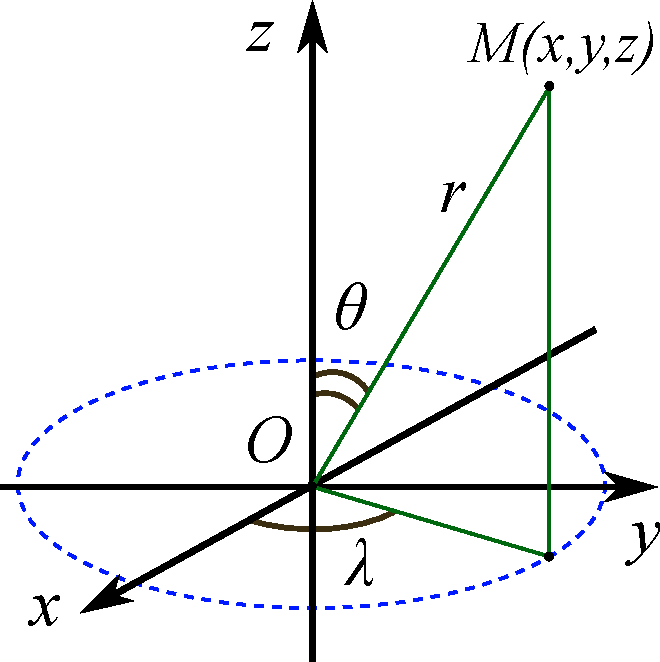
\includegraphics[width=0.45\linewidth]{../img/sphere_origin.pdf} & 
	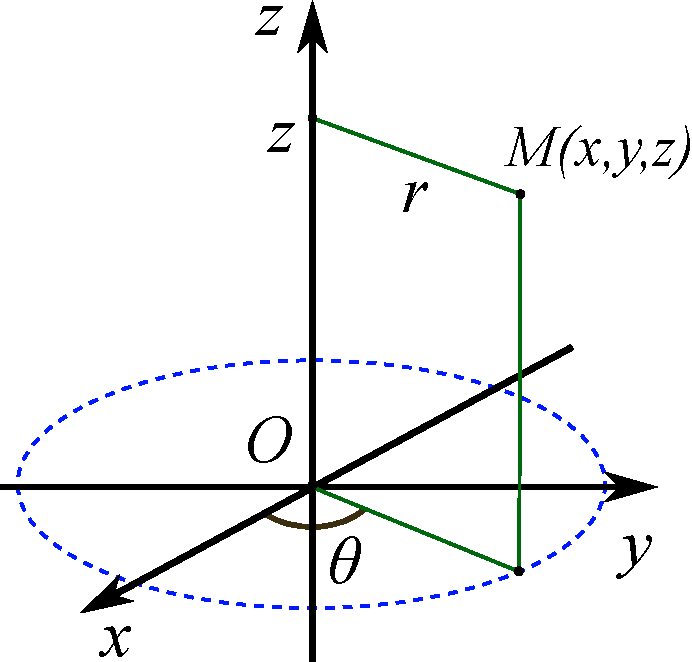
\includegraphics[width=0.45\linewidth]{../img/cylindrical_origin.pdf} \\
	а & б \\ 
	\end{tabular}
	\caption{Сферическая (а) и цилиндрическая (б) система координат}
	\label{fig:spherical_cylindrical_origin}
\end{figure}	


Уравнение неразрывности в цилиндрической системе координат ($r$, $\theta$, $z$)\footnote{В следствие симметрии пренебрегли зависимостью $\varphi$ от $\theta$.} (рис. \ref{fig:spherical_cylindrical_origin}б) в случае осесимметричного течения имеет вид:
\begin{equation}
\label{eq:mass_axis_symmetry_cylindrical}
\frac{1}{r}
\left\{
\pd{}{r}\left( r \pd{\varphi}{r} \right) + 
\pd{}{z}\left( r \pd{\varphi}{z} \right)
\right\}
= 0,
\end{equation}
где
\[
v_r = \pd{\varphi}{r},\quad
v_z =  \pd{\varphi}{z}.
\]

Из уравнение неразрывности в форме (\ref{eq:mass_axis_symmetry_cylindrical}) следует что
\[
	\pd{}{r}(r v_r)  = -\pd{}{z}(r v_z)
\]	
и существование полного дифференциала $\psi(r,z)$:
\[
	d\psi = r v_r dz - r v_z dr = \pd{\psi}{z} dz + \pd{\psi}{r} dr
\]


\begin{dfn}
Функцию $\psi\argrz$  такую, что
\[
	v_r = \displaystyle\frac{1}{r}\pd{\psi}{z},\quad
	v_z = -\displaystyle\frac{1}{r}\pd{\psi}{r},
\]
называют \alert{функцией тока для осесимметричных течений}.	
\end{dfn}

Уравнения линий тока в случае осесимметричного течения в цилиндрической системе координат:
\[
\frac{dr}{v_r} = \frac{dz}{v_z},
\]
следовательно на линиях тока:
\[
d\psi = r (v_r dz - v_z dr) = 0\quad
\Rightarrow\quad
\psi = const.
\]

Соотношения
\begin{equation}
	\label{eq:phi_psi_connection_sym}
	\pd{\varphi}{r} = \frac{1}{r}\pd{\psi}{z},\quad
	\pd{\varphi}{z} = -\frac{1}{r}\pd{\psi}{r}
\end{equation}
связывают функцию тока и потенциал для осесимметричных течений. Полученные соотношения \alert{отличаются} от условий Коши -- Римана (\ref{eq:Cauchi_Riman}), а уравнение для функции тока:
\[
	\pdk{\psi}{r}+\pdk{\psi}{z} - \frac{1}{r}\pd{\psi}{r} = 0
\]
не является уравнением Лапласа, записанным в цилиндрической системе координат. 
В случае осесимметричных течений не работают методы ТФКП. В этом случае может быть применен \alert{метод источников и стоков} и \alert{принцип суперпозиций}. 
		
Для моделирования течений, потенциалы которых известны применяется \textit{принцип суперпозиций}, заключающийся в следующем утверждении. Вследствие линейности уравнения неразрывности, если в области имеется несколько течений с потенциалами $\varphi_1(x,y)$, $\varphi_2(x,y)$, \ldots, $\varphi_n(x,y)$, то общий потенциал всего течения в заданной точке равен сумме потенциалов всех течений, присутствующих в области:
\[
\varphi(x,y) = \varphi_1(x,y) + \varphi_2(x,y) + \ldots + \varphi_n(x,y)
\] 		
или интегралу от распределенных потенциалов в некоторой области пространства.

Потенциалы и функции тока простейших осесимметричных течений в цилиндрических переменных ($r$, $z$):

\begin{enumerate}
	\item поступательное движение:
		\begin{equation}
			\label{eq:translation_3D}
			\varphi\argrz = V z \quad\Rightarrow\quad
			\psi\argrz = -\frac{V}{2}r^2 + C;
		\end{equation}
	\item  источник, сток:
		\begin{equation}
			\label{eq:source_3D}
			\varphi\argrz = -\frac{q}{4\pi} \frac{1}{\sqrt{r^2+z^2}}\quad\Rightarrow\quad
			\psi\argrz = \frac{q}{4\pi}\frac{z}{\sqrt{r^2+z^2}} + C;
		\end{equation}	
		\item диполь в направлении оси $Oz$:
			\begin{equation}
				\label{eq:dipol_3D}
				\varphi\argrz =  -\frac{M}{4\pi} \frac{z}{(\sqrt{r^2+z^2})^3}\quad\Rightarrow\quad
				\psi\argrz =  -\frac{M}{4\pi} \frac{r^2}{(\sqrt{r^2+z^2})^3}+C.
			\end{equation}
		
\end{enumerate}

\subsection{Задачи для самостоятельного решения}

\begin{problems}
	
	\item 
	Как преобразуются условия Коши-Римана в случае цилиндрических и сферических координат? Как выглядят операторы дифференциальных уравнений в постановке задач на потенциал и функцию тока (задачи Дирихле, Неймана)?
	
	\item Показать, что поток жидкости через поверхность, образованную вращением дуги, равен разности значений функции тока на концах этой дуги.
	
	\item Используя связь потенциала и функции тока (\ref{eq:phi_psi_connection_sym}), получить их выражения для элементарных течений, описывающих поступательное движение (\ref{eq:translation_3D}), источник (сток) (\ref{eq:source_3D}) и диполь (\ref{eq:dipol_3D}). Какое физическое значение у констант в этих формулах?
	
	\item 
	Для шара, двигающегося с ускорением в идеальной несжимаемой жидкости, определить силу, действующую на жидкость. \textit{Указание: воспользоваться уравнением Коши-Лагранжа после определения потенциала жидкости.}
	
	\item 
	Найти частоту колебаний шарика, находящегося в идеальной несжимаемой жидкости в случаях: 
	\begin{enumerate}
		\item шарик колеблется в плоскости, перпендикулярной вектору силы тяжести,
		\item шарик колеблется в поле силы тяжести.
	\end{enumerate}
	
	\item 
	Сферический пузырек всплывает в идеальной несжимаемой жидкости с плотностью $\rho$. Ускорение свободного падения $g$. Определить ускорение пузырька. Массой пузырька можно пренебречь.
	
	\item
	Сферический пузырек приводится в движение жидкостью. Ускорение жидкости вдали от пузырька равно $w$. Определить ускорение пузырька. Масса пузырька пренебрежимо мала, размер постоянен.
	
\end{problems}	

\section{Динамика вязкой жидкости}

\subsection{Реологическое уравнение состояния вязкой жидкости}

Компоненты тензора напряжения, определяющие динамические характеристики, связаны с компонентами тензора скоростей деформаций:
\begin{equation}
\label{eq:sigma_e_connection}
\sigma = -p I + 2 \mu e,
\end{equation}
где $\sigma$ -- тензор напряжений; $\mu$ -- коэффициент динамической вязкости; $I$ --  единичный тензор; $e$ -- тензор скоростей деформации;  $p$ -- давление.

Выражение (\ref{eq:sigma_e_connection})) имеет вид:
\begin{itemize}
	\item[--] в декартовой системе координат ($x_1$, $x_2$, $x_3$):
		\[
			\sigma_{ij} = -p\delta_{ij} + 2 \mu e_{ij}\quad (i,j = 1,2,3),	
		\]
		где
		\[
			\delta_{ij} = 
			\left\{
			\begin{array}{cl}
				1, & i = j,\\
				0, & i \neq j,\\
			\end{array}
			\right.\quad
			e_{ij} = \frac{1}{2}\left(
			\pd{v_i}{x_j}+\pd{v_j}{x_i}
			\right)
		\]
		\[
			(i,j = 1,2,3);
		\]
		
	\item[--] в сферической системе координат ($r$, $\lambda$, $\theta$) (рис. \ref{fig:spherical_cylindrical_origin}а):
	\[
	\sigma_{rr} = -p +2\mu\pd{v_r}{r},\quad 
	\sigma_{\lambda\lambda} = -p + 2\mu 
	\left(
		\frac{1}{r\sin\theta} \pd{v_\lambda}{\lambda} + \frac{v_r}{r} + \frac{v_\theta \ctg\theta}{r}
	\right),
	\]
	\[
	\sigma_{\theta\theta} = -p + 2\mu \left(
	\frac{1}{r} \pd{v_\theta}{\theta} + \frac{v_r}{r}
	\right),
	\]
	\[
	\begin{array}{l}
	\sigma_{r\theta} = \sigma_{\theta r} = \displaystyle \mu\left(
	\frac{1}{r} \pd{v_r}{\theta} + \pd{v_\theta}{r} - \frac{v_\theta}{r}
	\right), \\
	\sigma_{\lambda\theta} =  \sigma_{\theta\lambda}= \displaystyle \mu \left(
	\frac{1}{r\sin\theta} \pd{v_\theta}{\lambda} + \frac{1}{r}\pd{v_\lambda}{\theta} - \frac{v_\lambda \ctg\theta}{r}
	\right),\\
	\sigma_{\lambda r} =  \sigma_{r\lambda}= \displaystyle \mu \left(
	 \pd{v_\lambda}{r} + \frac{1}{r\sin\theta}\pd{v_r}{\lambda} - \frac{v_\lambda}{r}
	\right);
	\end{array}
	\]
	
	\item[--] в цилиндрической системе координат ($r$, $\theta$, $z$) (рис.~\ref{fig:spherical_cylindrical_origin}б):
	\[
	\sigma_{rr} = -p + 2 \mu \pd{v_r}{r},\quad
	\sigma_{\theta\theta} = -p + 2\mu \left( \frac{1}{r} \pd{v_\theta}{\theta} +\frac{v_r}{r} \right),\quad
	\sigma_{zz} = -p + 2\mu \pd{v_z}{z},
	\]
	\[
	\begin{array}{l}
		\sigma_{r\theta} = \sigma_{\theta r} = \displaystyle \mu\left(
		\frac{1}{r} \pd{v_r}{\theta} + \pd{v_\theta}{r} - \frac{v_\theta}{r}
		\right), \\
		\sigma_{\theta z} =  \sigma_{z\theta}= \displaystyle \mu \left(
		 \pd{v_\theta}{z} + \frac{1}{r}\pd{v_z}{\theta} 
		\right),\\
		\sigma_{zr} =  \sigma_{rz}= \displaystyle \mu \left(
		\pd{v_z}{r} + \pd{v_r}{z}
		\right).
	\end{array}
	\]
\end{itemize}

Для вычисления равнодействующей силы $\vec{F}$, со стороны вязкой жидкости на тело, ограниченное поверхностью $S$, необходимо вычислить следующий интеграл:
\[
\vec{F} = \int\limits_S \vec{n} \cdot \sigma \, dS,
\]
где $\vec{n}$ -- вектор внешней единичной нормали к поверхности $S$.


\subsection{Основные уравнения вязкой жидкости}

Движение вязкой несжимаемой жидкости описывается \alert{уравнениями Навье -- Стокса}:
\begin{equation}
	\label{eq:navier–stokes_mass}
	\divo \vec{v} = 0,
\end{equation}
\begin{equation}
	\label{eq:navier–stokes}
	\pd{\vec{v}}{t} + (\vec{v}\cdot\nabla)\vec{v} = -\frac{1}{\rho}\nabla p + \nu \Delta \vec{v} + \vec{f},
\end{equation}
где \alert{неизвестные функции}: $\vec{v}\argtxv$ -- вектор скорости; $p\argtxv$ -- давление; $T\argtxv$~-- температура. \alert{Константы и заданные зависимости}, определяющие течение: $\rho$ -- плотность; $\nu=\mu/\rho$ -- коэффициент кинематической вязкости; $\vec{f}$ -- вектор внешних сил. 
		
Расчёт температурного поля, если требуется осуществляется путём решения дополнительного уравнения, с использованием решения уравнений Навье-Стокса:
\[
c_V\left(\pd{T}{t} + (\vec{v}\cdot\nabla)T \right) = \frac{\kappa}{\rho} \Delta T + \frac{2\mu}{\rho} e_{ij}e_{ij},
\]
\[
e_{ij} = \frac{1}{2}\left(
\pd{v_i}{x_j}+\pd{v_j}{x_i}
\right)\quad
(i,j = 1,2,3),
\]
где $e_{ij}$ -- тензор скоростей деформации ($i,j = 1,2,3$); $\kappa$ -- коэффициент температуропроводности.

В случае \alert{осесимметричного течения} уравнения Навье-Стокса имеют вид:
\begin{itemize}
	\item[--] в цилиндрической системе координат ($r$, $\theta$, $z$) (рис. \ref{fig:spherical_cylindrical_origin}б) \footnote{Пренебрегли зависимостью от $\theta$.}:
\[
\pd{}{r} (r v_r) + \pd{}{z} (r v_z) = 0,
\]
\[
\pd{v_r}{t} + v_r\pd{v_r}{r} + v_z\pd{v_r}{z} = -\frac{1}{\rho} \pd{p}{r} + \nu \left(\Delta v_r - \frac{v_r}{r^2}\right),
\]
\[
\pd{v_z}{t} + v_r\pd{v_z}{r} + v_z\pd{v_z}{z} = -\frac{1}{\rho} \pd{p}{z} + \nu \Delta v_z,
\]
\[
\Delta = \pdk{}{r}+\frac{1}{r}\pd{}{r} + \pdk{}{z};
\]
	\item[--] в сферической системе координат ($r$,  $\lambda$, $\theta$) (рис. \ref{fig:spherical_cylindrical_origin}а)\footnote{Пренебрегли зависимостью от $\lambda$.}:
\[
\frac{1}{r^2} \pd{}{r}(r^2 v_r) + \frac{1}{r \sin \theta} \pd{}{\theta}(v_\theta \sin\theta) = 0,
\]
\[
\pd{v_r}{t} + v_r\pd{v_r}{r} + \frac{v_\theta}{r} \pd{v_r}{\theta} - \frac{v_\theta^2}{r} = -\frac{1}{\rho} \pd{p}{r} + 
\nu \left(\Delta v_r - \frac{2 v_r}{r^2} - \frac{2}{r^2}\pd{v_\theta}{\theta} - \frac{2 v_\theta \ctg\theta}{r^2}\right),
\]
\[
\pd{v_\theta}{t} + v_r\pd{v_\theta}{r} + \frac{v_\theta}{r} \pd{v_\theta}{\theta} + \frac{v_r v_\theta}{r} = 
-\frac{1}{r \rho} \pd{p}{\theta} + 
\nu \left(\Delta v_\theta + \frac{2}{r^2}\pd{v_r}{\theta} - \frac{v_\theta}{r^2 \sin^2 \theta}\right),
\]
\[
\Delta = \frac{1}{r^2} \pd{}{r}\left(r^2\pd{}{r}\right) + \frac{1}{r^2 \sin\theta} \pd{}{\theta} \left(\sin\theta \pd{}{\theta}\right).
\]
\end{itemize}

\subsection{Постановка граничных условий в контактных задачах вязкой жидкости}

При исследовании обтекания твёрдых тел вязкой жидкостью необходимо использовать условие \alert{прилипания}, заключающееся в том, что скорость жидкости на границе с телом совпадает со скоростью перемещения границы. Если тело покоится, то скорость жидкости равна нулю.

На \alert{контактном разрыве} необходимо также ставить динамическое условие, заключающееся в равенстве напряжений, возникающих на касательной к разрыву площадке.

Для течения вязкой жидкости и идеального газа (рис.~\ref{fig:viscous_fluid_gas}) без учёта сил поверхностного натяжения ставятся следующие условия.

\alert{Кинематическое} условие:
\[
v_n|_S = u_n,
\]
где $S$ -- поверхность контактного разрыва; $v_n$ -- нормальная составляющая скорости жидкости на границе; $u_n$ -- нормальная составляющая скорости газа на границе; $\vec{n}$ -- вектор нормали к поверхности.

\alert{Динамические} условия:
\[
(\vec{n}\cdot\sigma)\cdot\vec{n}|_S= p|_S = p_0,
\]
\[
(\vec{n}\cdot\sigma)\cdot\vec{\tau}|_S = 0,
\]
где $\sigma$ -- тензор напряжений в вязкой жидкости; $p_0$ -- давление газа; $\vec{\tau}$ -- касательный вектор к поверхности.

\begin{figure}
	\centering
	\begin{tabular}{c}
		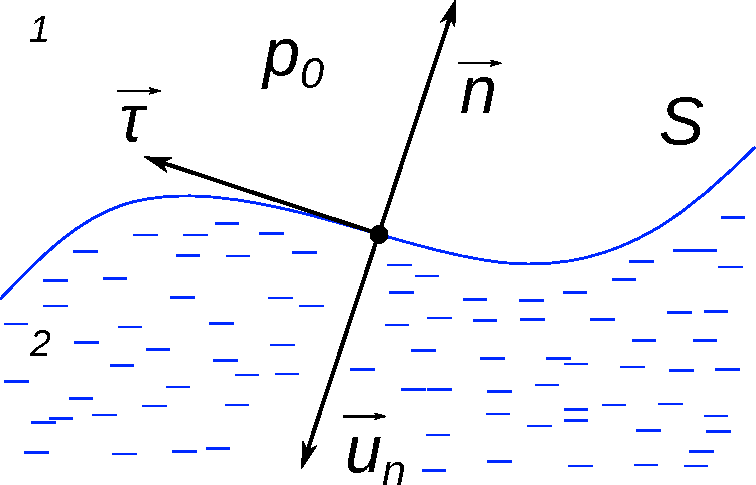
\includegraphics[width=0.6\linewidth]{../img/free_bound} \\
	\end{tabular}
	\caption{Пример течения с контактным разрывом для вязкой жидкости и идеального газа: 1 -- идеальный газ; 2 -- вязкая жидкость}
	\label{fig:viscous_fluid_gas}
	
\end{figure}	

\subsection{Коэффициенты подобия при течениях вязкой несжимаемой жидкости}

Используя замену переменных 
\[
t = T t',\quad
x = L x',\quad 
y = L y',\quad
z = L z',			
\]
\[
\vec{v}\argtxyz = V \vec{v}'\argtxyztick,\quad
\vec{f}\argtxyz = F \vec{f}'\argtxyztick
\]
\[
p\argtxyz = P p\argtxyztick',
\]
где $T$, $L$, $V$, $P$, $F$ -- характерные значения времени, размера течения, скорости, давления, силы сплошной среды, а штрихованные параметры -- это новые безразмерные переменные, уравнения Навье-Стокса (\ref{eq:navier–stokes}) приводится к следующему виду:
\begin{equation}
\label{eq:Navier-Stokes_dim}
\Sh\pd{\vec{v'}}{t'} + (\vec{v}' \cdot \nabla') \vec{v'} = \frac{1}{\Fr} \vec{f'}  - \Eu \nabla' p' + 
\frac{1}{\Re} \Delta' \vec{v}',
\end{equation}
где $\nabla'$ и $\Delta'$ -- операторы градиента и Лапласа по штрихованным переменным.

\begin{dfn}
		Безразмерные комплексы, обуславливающие течения вязкой жидкости, являются критериями подобия и имеют следующие названия:
		\[
		\begin{tabular}{ll}
			$\displaystyle\frac{L}{VT} = \Sh$ -- число Струхаля, & $\displaystyle\frac{P}{\rho V^2}=\Eu$ -- число Эйлера, \\
			$\displaystyle\frac{VL}{\nu} = \Re$ -- число Рейнольдса, & $\displaystyle\frac{V^2}{F L}=\Fr$ -- число Фруда.
		\end{tabular}
		\]
\end{dfn}

Число Струхаля $\Sh$ определяет насколько течение можно считать установившимся (стационарным), число Рейнольдса $\Re$~-- вклад  вязких членов по сравнению с инерционными, число Эйлера $\Eu$~-- вклад градиента давления по сравнению с напором, число Фруда $\Fr$~-- вклад внешнего поля.

\subsection{Приближение Стокса и ползущие течения}

\begin{dfn}
Течения, для которых число Рейнольдса много меньше $1$:
\[
	\Re= \frac{L V \rho}{\mu} \ll 1,
\]
называются ползущими течениями.
\end{dfn}

Произведём оценку вклада конвективного слагаемого по сравнению с вязким в уравнениях Навье -- Стокса (\ref{eq:navier–stokes}) для ползущего течения:
\[
\frac{\rho |(\nabla\cdot\vec{v})\vec{v}| }{\mu |\Delta\vec{v}|} \sim 
\frac{\rho V^2}{L} : \frac{\mu V }{(L)^2} = \Re \ll 1.
\]

Отбрасывая \alert{нелинейные инерционные члены} $(\nabla\cdot\vec{v})\vec{v}$ в (\ref{eq:navier–stokes}), получим линейное приближение \alert{Стокса} уравнений (\ref{eq:navier–stokes_mass}), (\ref{eq:navier–stokes}):
\begin{equation}
\label{eq:Stokes}
\divo \vec{v} = 0,\quad
\nabla p = \mu \Delta\vec{v}.
\end{equation}
	
\subsection{Задачи для самостоятельного решения}

\begin{problems}
	
	\item Найдите вектор скорости, давление, вектор вихря и силу Стокса при обтекании шара вязкой жидкостью в приближении Стокса.
	
	{\small
	\textit{Указание.}	
	
	Решение (поиск констант) предлагается искать следующим образом: подействуйте ротором на уравнение количества движения в приближении Стокса, что приведёт к уравнению на вектор вихря, затем воспользуйтесь соображением симметрии для вектора вихря, далее, найдите вектор вихря с точностью до константы, решая дифференциальное уравнение, затем, пользуясь уравнением неразрывности и разложением в ряд для скоростей в сферических координатах (по расстоянию от центра шара), найдите компоненты скоростей с учетом граничного условия. Определив давление, найдите силу Стокса.  \newline		
	Решение  также можно искать следующим образом: подействуйте оператором дивергенции на уравнение количества движения с целью выделения уравнения на давление. Это даст множество решений, но из лекции мы знаем какое взять. Почему член  не входит в выражение для давления? Помимо условий на границе шара, используйте уравнение неразрывности для получения условий на неизвестные константы. При нахождении констант не забудьте также про константу при давлении. Почему член  не входит в выражение для скорости? Почему член  входит в выражение для скорости и к чему это приводит (относительно обтекания сферы идеальной жидкостью посмотреть)? Как симметрия задачи оказывает влияние на составление членов, потенциально подходящих под решение?
	}

	\item 
	Проанализировать поведение найденного поля скоростей при отдалении от шара. Почему наблюдается такое поведение скоростей? Что следует сделать, чтобы уточнить полученное решение? 
	
	\item
	Показать, что в вязкой жидкости происходит диссипация энергии.
	 
	{\small \textit{Указание:} показать, что работа, совершаемая над жидкостью, не целиком идёт на изменение кинетической энергии.}

\end{problems}

\section{$\Pi$-теорема}

\subsection{Определения и примеры}

\begin{dfn}
	Два физических явления называются \alert{подобными}, если величины, характеризующие одно явление, могут быть получены из соответствующих величин другого, взятых в сходственных пространственно-вре\-мен\-ных точках, простым умножением на \textit{одинаковые во всех точках множители}, называемые \textit{коэффициентами подобия}.
\end{dfn}

Примером подобия может служить система уравнений Навье-Стокса, записанная в безразмерных переменных (\ref{eq:Navier-Stokes_dim}). Критериями подобия являются безразмерные комплексы: число Рейнольдса $\Re$, число Фруда $\Fr$, число Струхаля $\Sh$, число Эйлера $\Eu$. Все обезразмеренные решения уравнений (\ref{eq:navier–stokes}) будут являться функциями от этих безразмерных комплексов.

Для того чтобы использовать теорию размерности необходимо ввести понятие \alert{размернооднородной} функции. 

\begin{dfn}
	Функция $f(x_1, x_2, \ldots, x_n)$ называется \alert{размернооднородной}, если существует такая совокупность чисел $b_k$ ($k=\overline{1,m}$), что имеет место равенство
	\begin{equation}
	\label{eq:dimension_uniform_function_dfn}
	f(\alpha_1^{a_{11}}\ldots \alpha_m^{a_{1m}}x_1,\ldots,
	\alpha_1^{a_{n1}}\ldots \alpha_m^{a_{nm}}x_n) = 
	\alpha_1^{b_1}\alpha_2^{b_2}\ldots \alpha_m^{b_m} f(x_1, x_2, \ldots, x_n)
	\end{equation}
	для всех $\alpha_k$ ($k=\overline{1,m}$) и $x_i$ ($i=\overline{1,n}$) в области определения.
\end{dfn}

Рассмотрим классическую задачу колебания математического маятника, представляющего собой механическую систему, состоящую из материальной точки на конце невесомой нерастяжимой нити или лёгкого стержня и находящуюся в однородном поле сил тяготения. Известно, что период его колебания определяется формулой:
\[
T(l, g) = 2 \pi \sqrt{\frac{l}{g}},
\]
где $T$ -- период колебания, с; $l$ -- длина, м; $g$ -- ускорение свободного падения, м/с$^2$.

Пусть длина нити $l = x_1$~м, ускорение свободного падения $g = x_2$~м/c$^2$. Коэффициенты $\alpha_i$ ($i=1,2$) -- это коэффициенты пересчёта параметров из одной системы единиц в другую (например, связанной с метрами и секундами в систему единиц, связанную с километрами и минутами, т.е. $\alpha_1 = 10^{-3}$~км/м, $\alpha_2 = 60^{-1}$~мин/с).

Период колебаний маятника $T$ является размернооднородной функцией, т.к. равенство
\begin{equation}
\label{eq:T_dim_connection}
T(\alpha_1 x_1, \alpha_1 \alpha_2^{-2} x_2) = 2 \pi \sqrt{\frac{\alpha_1 x_1}{\alpha_1 \alpha_2^{-2} x_2}} = \alpha_2 T(x_1, x_2)
\end{equation}
выполнено для всех $x_i$, $\alpha_j$ ($i,j=1,2$) в области определения. В данном случае $b_1 = 0$, $b_2 = 1$. 

Для указанных значений $\alpha_i$ выражение (\ref{eq:T_dim_connection}) связывает период колебания маятника в часах, через параметры выраженные в системе единиц СИ.


Следующая теорема позволяет использовать теорию размерностей для уменьшения числа зависимых переменных размерооднородной функции, используя безразмерные комплексы от этих параметров.


\begin{theorems}{[$\Pi$-теорема (Бекингем, Федерман)]}
Если $x_1$, $x_2$, \ldots, $x_n$ -- численные значения $n$ физических величин, $A=(a_{ij})$ ($i=\overline{1,n}$, $j=\overline{1,m}$) -- матрица их размерностей по отношению к единицам измерения $M_1$, $M_2$,\ldots, $M_m$, $f$ -- произвольная размернооднородная функция переменных  $x_1$, $x_2$, \ldots, $x_n$, а $\Pi_1$, $\Pi_2$, \ldots, $\Pi_p$ ($p=n-r$, $r$ -- ранг матрицы $A$) -- фундаментальная система степенных одночленов переменных $x_1$, $x_2$, \ldots, $x_n$, то при произвольных действительных числах $k_1$, $k_2$, \ldots, $k_n$ имеет место равенство
\[
f(x_1, x_2, \ldots, x_n) = x_1^{k_1} x_2^{k_2} \ldots x_n^{k_n}
G(\Pi_1, \Pi_2, \ldots, \Pi_p).
\]
\end{theorems}

Выведем формулу периода колебания маятника из соображений размерностей, используя $\Pi$-теорему. В данном случае $n=2$ -- количество неизвестных параметров (длина нити и ускорение свободного падения) и $m=2$ -- количество независимых размерностей (метры и секунды). Тогда $2 \times 2$ матрица $A$ размерностей будет иметь вид:
\[
\begin{array}{c||c|c}
& \text{м} &  \text{с} \\
\hline
\hline
l & 1 & 0 \\
\hline
g & 1 & -2 \\
\end{array}
\]
Ранг матрицы $A$  $r=2$. Безразмерных комплексов, от которых зависит функция $G$, будет $p=n-r=2-2=0$. Таким образом, по $\Pi$-теореме:
\[
T(l,g) =  l^{k_1} g^{k_2} G_0,
\]
где $G_0$ -- безразмерная константа; $k_1$, $k_2$ -- показатели степени.
$k_1$, $k_2$ выбираются из соображения, чтобы обезразмерить целевую функцию $T$. 

В данном случае $k_1 = 1/2$, $k_2 = -1/2$ и 
\[
T(l,g) = G_0 l^{1/2} g^{-1/2}= G_0  \sqrt{\frac{l}{g}},
\]
т.к. $\text{м}^{1/2} \cdot \left(\displaystyle\frac{\text{м}}{\text{с}^2}\right)^{-1/2} = \text{с}$.

Величину $G_0$ необходимо уточнить из дополнительных соображений (например, эксперимента).

\subsection{Задачи для самостоятельного решения}

\begin{problems}
	
	\item Используя $\Pi$-теорему, определить силу сопротивления шара при его внедрении с постоянной скоростью $v$ в полупространство, заполненное вязкой несжимаемой жидкостью. Рассмотреть предельные случаи $v \to 0$, $v \to \infty$. Радиус шара известен.
	
	\item
	Используя  $\Pi$-теорему, определить силу сопротивления, действующую на шар, движущийся в вязкой, несжимаемой бесконечной жидкости. Рассмотреть предельные случаи $v \to 0$, $v \to \infty$. Основные параметры системы считать заданными.
	
	\item
	Задача о точечном взрыве. В некоторой точке выделилось количество энергии $E$ . Определить зависимости скорости $D$ и координаты $R$ ударной волны от времени $t$, а также скорость $v_2$, плотность $\rho_2$ и давление $p_2$ за ударной волной. 

\end{problems}

\section{Одномерные изоэнтропические течения идеального газа }

\subsection{Задачи для самостоятельного решения}

\begin{problems}
	
	\item Пользуясь методом характеристик, повторить вывод инвариантов Римана и характеристических направлений на основе изоэнтропического приближения одномерной газовой динамики.
	
	\item
	В момент $t=0$  покоящийся газ с параметрами $v_0 = 0$, $p_0$, $\rho_0$ находится в трубе при $x<0$. Справа в трубе вакуум. Найти $v(x,t)$, $\rho(x,t)$, $p(x,t)$, $T(x,t)$, $c(x,t)$ при истечении газа в вакуум. Сравнить полученную максимальную скорость истечения газа c максимальной скоростью истечения газа в вакуум в стационарном случае.
	
	\item 
	В цилиндр, заполненный покоящимся воздухом с параметрами $v_0 = 0$, $\rho=\rho_0$, $p=p_0$, вдвигается поршень с постоянным ускорением $a$. Найти момент возникновения ударной волны $t^*$.
	
	\item
	Определить закон движения поршня площадью $S$ и массой $m$, выталкиваемого газом с начальными параметрами $v_0=0$, $p_0$, $\rho_0$ в вакуум (см. иллюстрацию).

	\begin{figure}[h!]
		\centering
		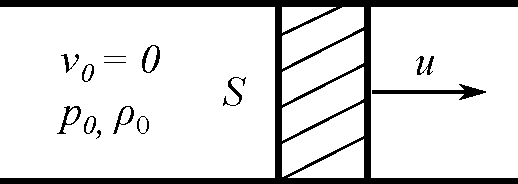
\includegraphics[width=0.5\textwidth]{../img/piston_u.pdf}
	\end{figure}
	
	\item 
	Из трубы, заполненной при $x>0$ газом с параметрами  $v_0=0$, $p_0$, $\rho_0$, начинает выдвигаться поршень с постоянной скоростью $u$. Определить движение газа.

\end{problems}

\end{document}